\chapter{Interface Design} % Main chapter title

\label{Chapter6} % For referencing the chapter elsewhere, use \ref{Chapter1} 

\lhead{Chapter 6. \emph{Interface Design}} % This is for the header on each page - perhaps a shortened title

%----------------------------------------------------------------------------------------
This section provides detailed illustration of the non-interactive
(map animation) and interactive dynamic energy map implementation and
design choices regarding the interactive dynamic energy map. The
section starts with a general overview that explains possible
approaches to add the time dimension in an energy map. Then the
non-interactive energy map (map animation) approach is presented. For
the non-interactive animation, the advantages and disadvantages
between different symbol or color representation on the effectiveness
of conveying information was briefly discussed.

Next a detailed documentation of the dynamic energy map interface is
presented. The layout and functions of each components of the
interface is explained and the design of each component based on
literature studies of dynamic map design is discussed. The use of
dynamic energy map to identify energy recovery opportunities and to
help design and size a district energy system is demonstrated.

\section{Overview}

Dorling and Openshaw pointed out that a dynamic map provides new
potential and possibilities for data analysis but also poses a great
challenge as a result of the less developed theory in space-time
pattern detection and measurement~\cite{Dorling1992}. In order to
better conduct a space-time visualization of the space-time energy
demand information in the dynamic energy map,literature studies on
space-time map visualization were used to design the dynamic energy
map.

Brownrigg mentions several methods of representing time on a map: 1) a
graph or chart that represents a function over time or a time line for
displaying chronological events 2) a sequence of snapshots displayed
over time (animated map) 3) small-multiples of snapshots of changing
states ~\cite{Brownrigg2005}.

Based on the classification above, method 1) and 2) were applied to
represent time for the dynamic energy map. The dynamic plot of
temporal time series uses method 1) to anchor the quantitative
information. The sequential map image display is using method 2). The
researcher did not use the small multiple method (method 3)). The
choice is based on the following points mentioned by Brownrigg: 1) the
number of snapshots in one display is limited and the finer the detail
per snapshot, the less snapshots one can contain in one display. Since
the 3D representation is chosen as one of the major map display
methods (2D map is also available), the level of details per image is
relatively high. This will result in a very small number of multiples
per display~\cite{Brownrigg2005} 2) the subtle changes are easier to
be noticed in the form of animation than with small-multiples
~\cite{Brownrigg2005}. Both drawbacks of small-multiple method will
impair the ability to convey the rapid temporal changes of community
energy behavior, hence is not suitable for the current project.

\section{(Non-interactive) Map Animation} \label{anime} 

Map animation was introduced to cartography in
1930s~\cite{Harrower2008}. Its major application include: 1)
demonstrating the dynamic process of geographic events (weather maps
in weather forecasting is such an example) 2) assisting pattern
recognition and knowledge development for scientific researches. The
study by Dorling and Openshaw is an example of application 2), where
they discovered new leukaemia hotspots through animated
maps~\cite{Dorling1992}.  Animated maps are proven to be more powerful
in conveying the spatial-temporal pattern than static
maps~\cite{McEachern1998}.

The level of user control of playback behavior of animated maps is
debatable. Providing the full freedom of adjusting the playback can
enhance pattern understanding~\cite{Nelson1998}, but it might also
reduce time animation to still images and impair its ability in
conveying temporal changes ~\cite{Lowe2004}. In the current dynamic
map project. The researcher observed that the non-interactive map
animation is especially helpful in conveying the dynamic energy
changing and the non-coincident peak arriving time of different
buildings in the community. Resch et al.\ suggest that the interface
for general public should ``ensure that the amount of information
shown to the users at any given time, and its complexity, are
reduced''~\cite{Resch2014}. The non-interactive animated map could be
one of the potential choices for an interface of a dynamic energy map
with general public as the target user group.

For this project a continuous color encoding method was used in the
creation of non-interactive animation of a univariate gas heating
energy demand map. Similar to the National Heat Map, the Calgary Map
and the EMIOFN project (\tref{tab:mapRep}) discussed in
\sref{sec:mapRepre}, a red to blue color ramp is used in the map
display. Different from the cases above, the current project chose to
represent high heat demand with blue and low heat demand with red as a
result of a limited survey of potential users. Each color within this
red-to-blue color scheme is represented as a real number between 0 and
1 with 0 representing pure red and 1 representing pure blue.

The first approach to calculate the corresponding color for each
heating energy value is to calculate the normalized distance between
the current value and the maximum value (\eref{eq:linear}).

\begin{equation}\label{eq:linear}
  {E(t) – E_{max} \over E_{max}}
\end{equation}

$E(t)$ is the energy consumption for the current time spot $t$,
$E_{max}$ is the maximum energy consumption over the year. The problem
for this approach is that the color changing is not visible enough as
a result of a extremely right skewed energy data (with each data point
representing the hourly energy consumption of a certain building in
the community at a certain hour of a year) distribution
(\fref{fig:heatOri}).

\begin{figure}[h!]
  \centering
  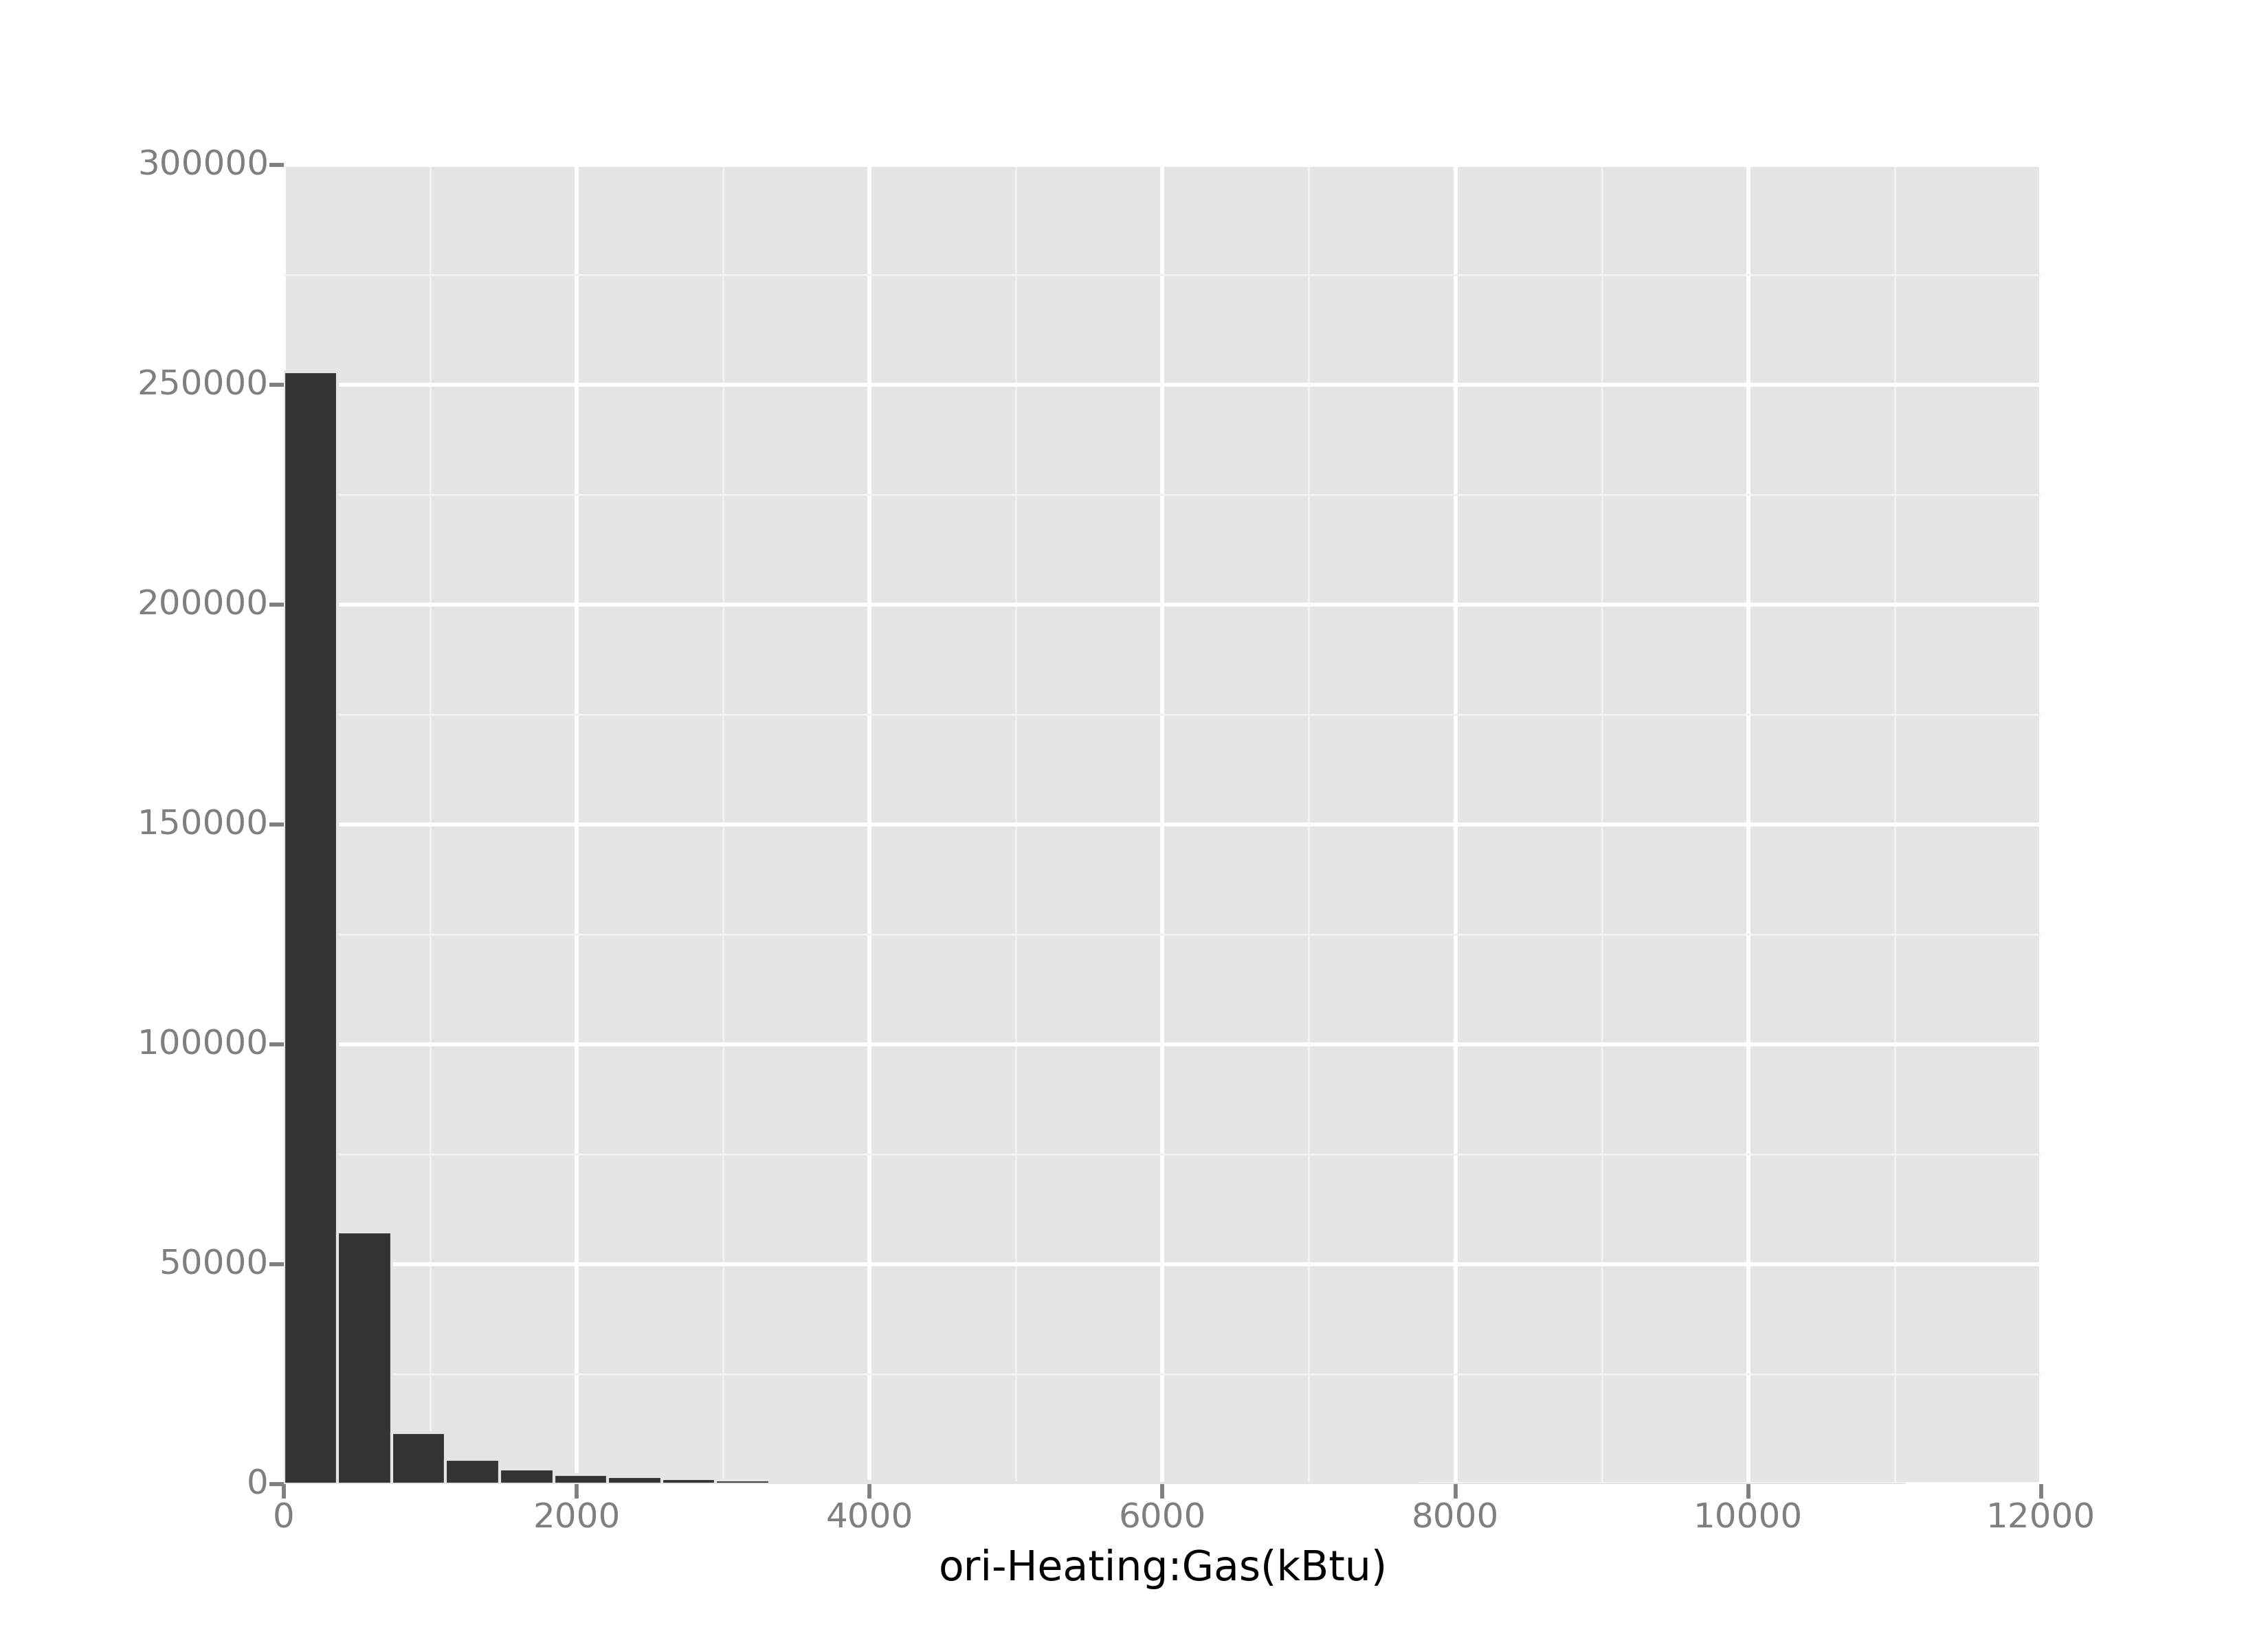
\includegraphics[width=0.7\linewidth]{heatOri.png}
  \caption[Heating Demand Histogram of Conceptual City]{A histogram of
    hourly energy consumption per building, for the 68 buildings in
    the community}
  \label{fig:heatOri}
\end{figure}

By directly applying this normalized color scheme, the color
distribution on a map will be very un-even, with most of the buildings
colored with the red color for most of the time.

Kolter and Ferreira discovered that the annual total energy
consumption of the 6500 buildings in Cambridge MA area follows a
``log-normal'' distribution~\cite{Zico2011}. By applying similar log
scaling for the hourly heating energy data of the community, the researcher found
that the hourly heating energy distribution also roughly follows a
normal distribution (\fref{fig:heatLog}). the researcher apply log scaling to
flatten the distribution and calculate the color from energy
($E(t)$) as follows:

\begin{equation}\label{eq:log}
  {\ln(E(t)) – \ln(E_{max}) \over \ln(E_{max})}
\end{equation}

\begin{figure}[h!]
  \centering
  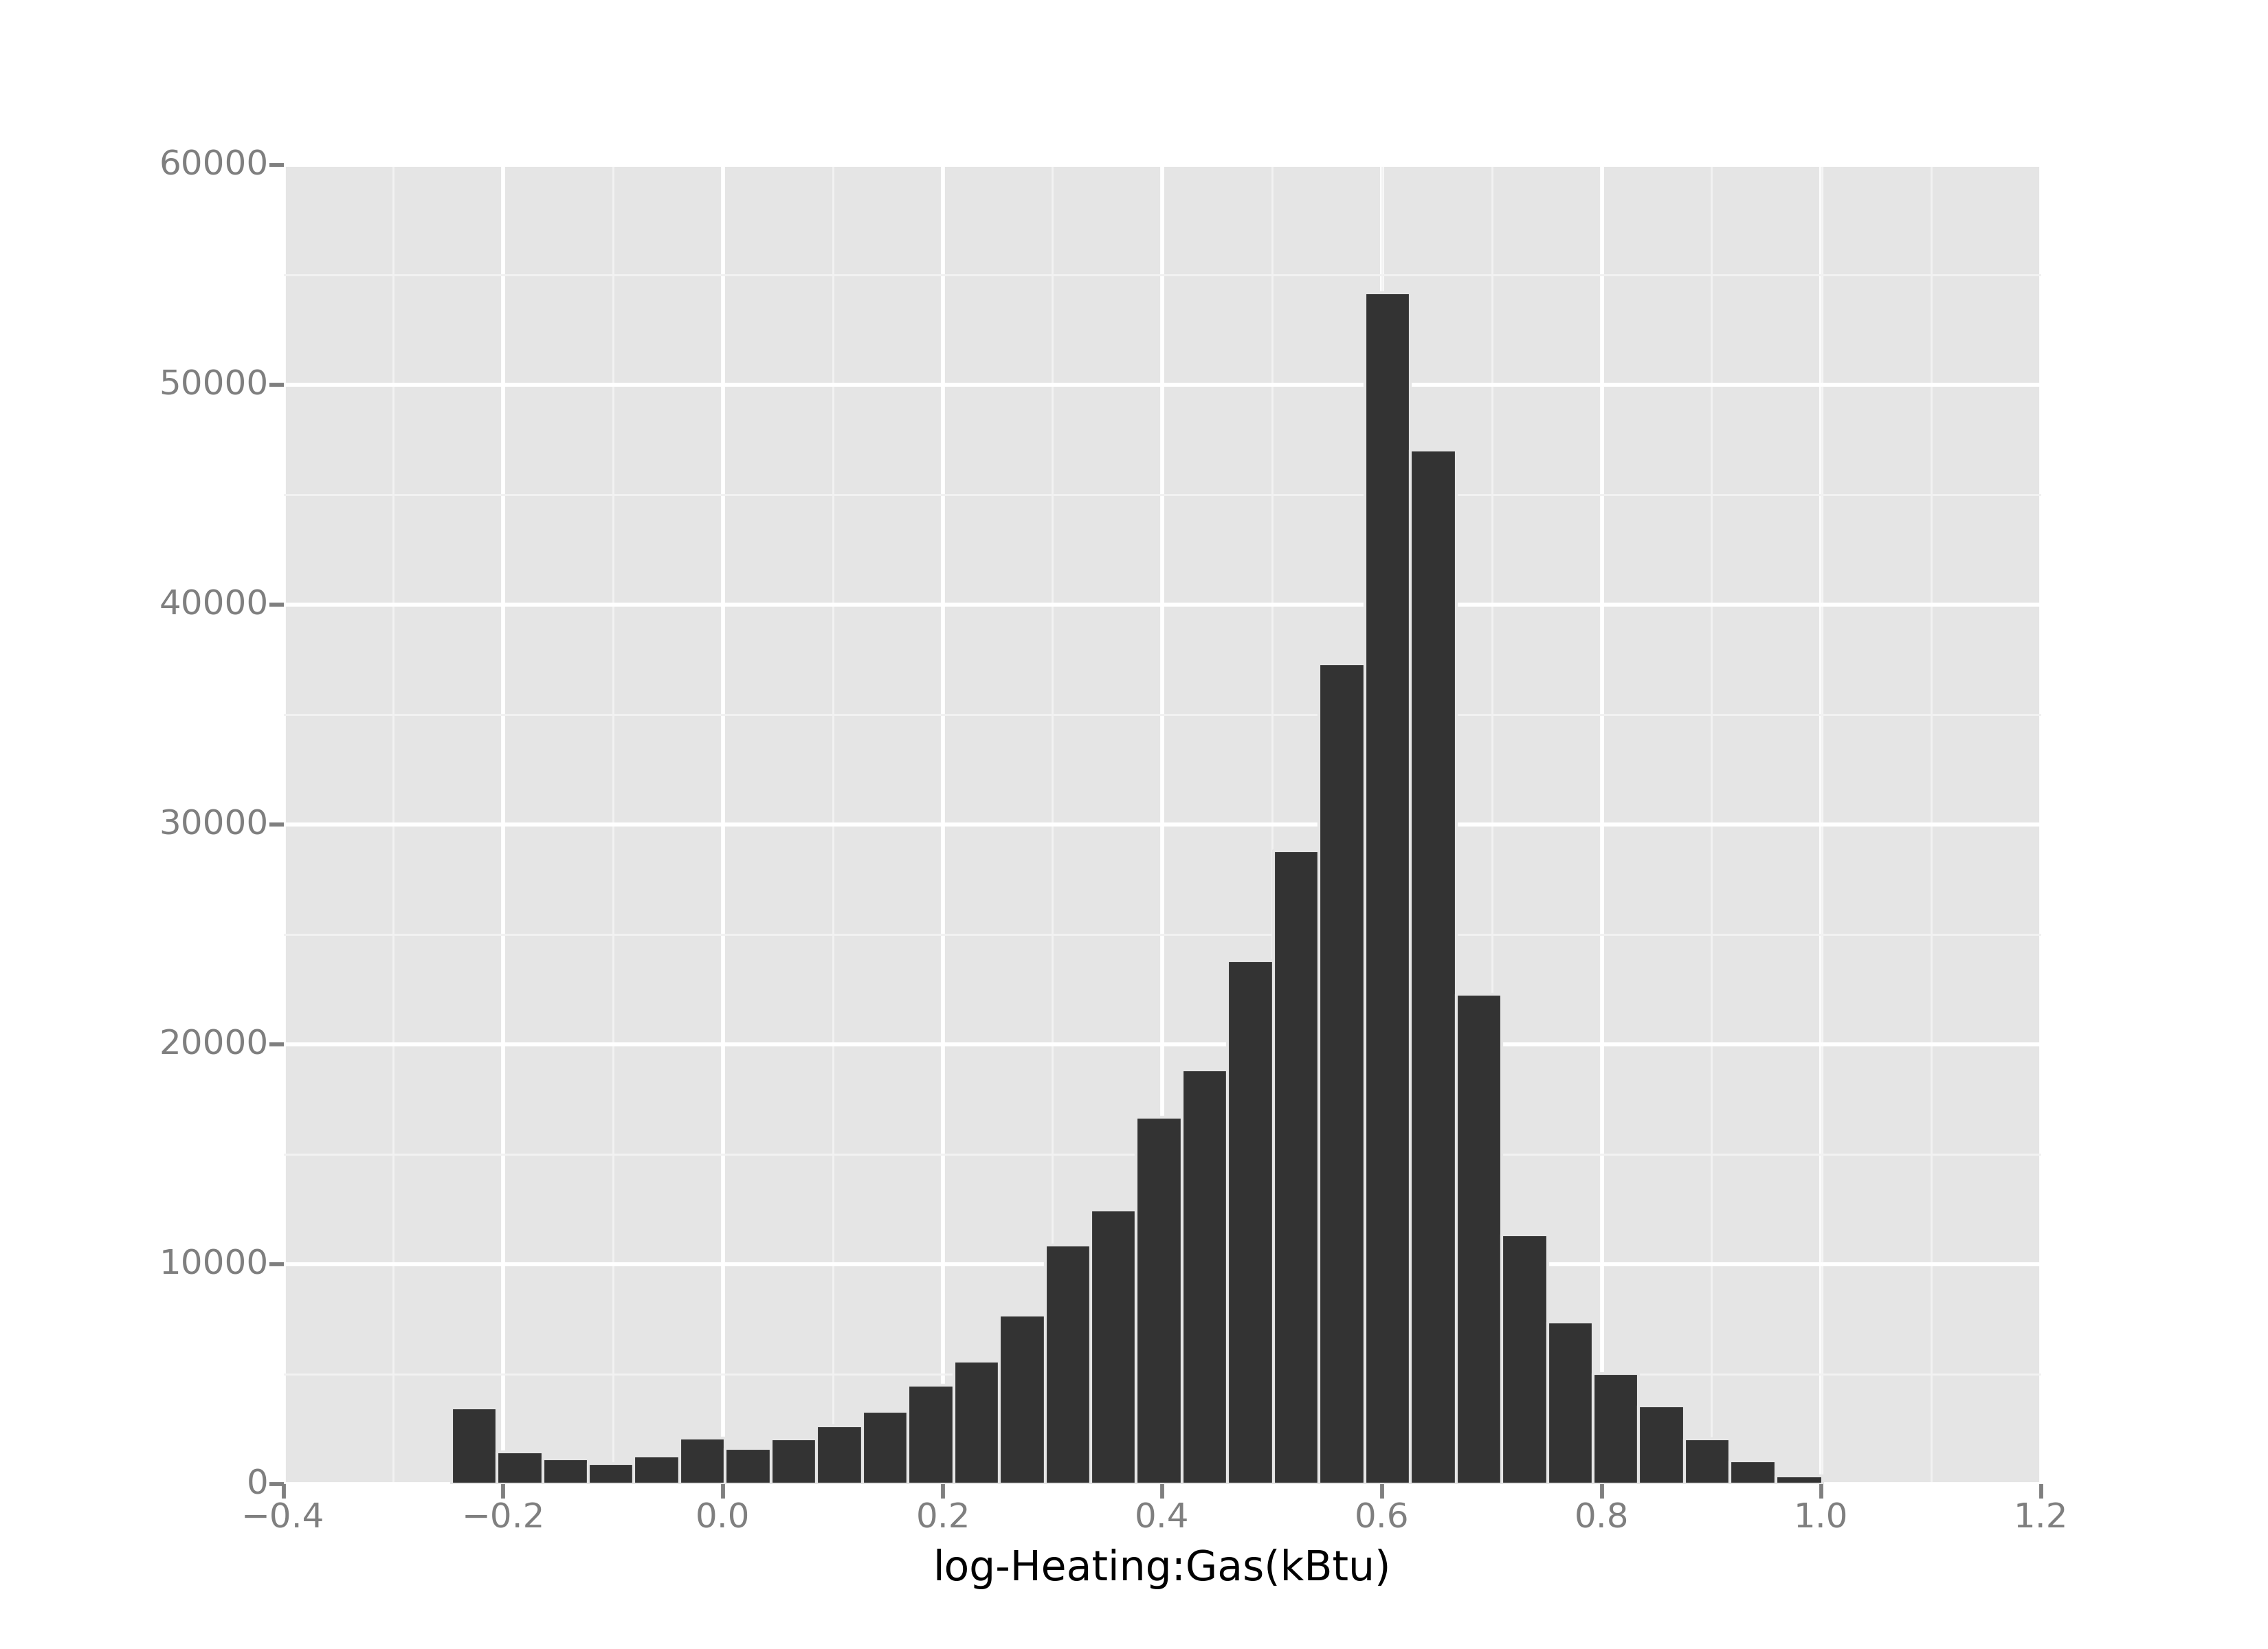
\includegraphics[width=0.7\linewidth]{heatLog.png}
  \caption[Heating Demand of Conceptual City]{Heating Demand of
    Conceptual City}
  \label{fig:heatLog}
\end{figure}

\fref{fig:img0002} is one snapshot of the conceptual urban environment
model under the log scaled calculation method in \eref{eq:log}.
\begin{figure}[h!]
  \centering
  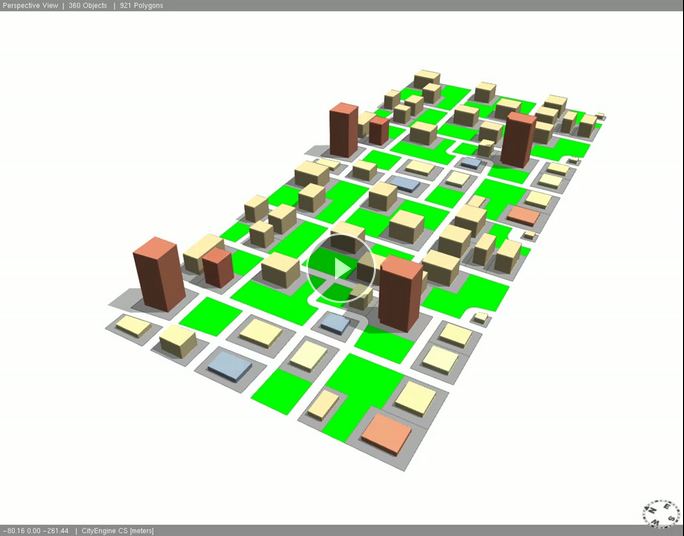
\includegraphics[width=0.7\linewidth]{img0002.png}
  \caption[Animation Demo of the Color Calculation]{Animated
    demonstration of the log-scaled dynamic energy heating demand map}
  \label{fig:img0002}
  \href{http://www.armechxyj.com/energy-mapping.html/#colorAnime}{Click
    here to go to the animation link}.
\end{figure}

In the dynamic energy map interface design, the researcher applied a
discrete color encoding with a seven-class bivariate choropleth
representation (\tref{tab:breakpoint}). The break points are
calculated purely with the Quantile method in
\sref{dataClassification}. This allows for a quantitative legend that
can depict more specific energy demand information. An animation with
this discrete color scheme is also created and can be viewed and
downloaded
\href{http://www.armechxyj.com/energy-mapping.html#redblueAnime3d}{through
  this link}.

\begin{table}[]
\centering
\caption{Heating-Cooling Breakpoints in the Interface}
\label{tab:breakpoint}
\begin{tabular}{rr|rr}
  \hline
heating &      & cooling &     \\
  \hline
  \hline
kBtu    & Ton  & kBtu    & Ton \\
5       & 60   & 2       & 24  \\
22      & 264  & 7       & 84  \\
50      & 600  & 15      & 180 \\
91      & 1092 & 26      & 312 \\
136     & 1632 & 56      & 672 \\
213     & 2556 & 72      & 864\\
  \hline
\end{tabular}
\end{table}

Although the initial conditions of the map instances using the
continuous and discrete encoding method are different: the animation
with continuous color encoding depicts only one variable (gas heating)
while the animation with discrete color encoding depicts two variables
(space heating and cooling), the researcher observed that the
continuous color encoding method seems to be better in demonstrating
the general pattern of energy changing behavior. Further evaluations
are needed to compare these two approaches and justify the design
choice of a discrete or continuous color scheme.
\section{Interactive Dynamic Map Interface}
\subsection{General Layout}
The general layout of the dynamic map interface is displayed in
\fref{fig:interfaceLayout}. It contains the following major sections :
\begin{figure}[h!]
  \centering
  \begin{subfigure}{0.7\textwidth}
  \centering
  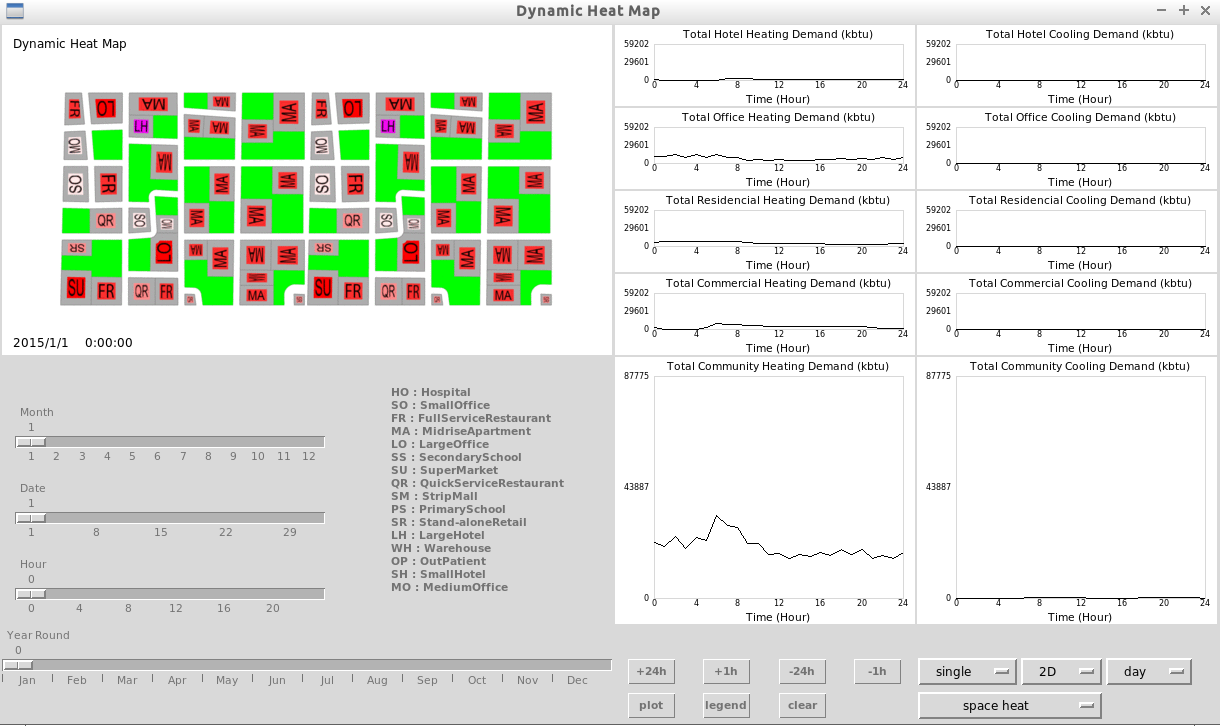
\includegraphics[width=\linewidth]{interface08}
  \caption[Dynamic Energy Map Interface Snapshot]{A snapshot of the dynamic energy map interface}
  \label{fig:interface08}
\end{subfigure}
~
\begin{subfigure}{0.7\textwidth}
  \centering
  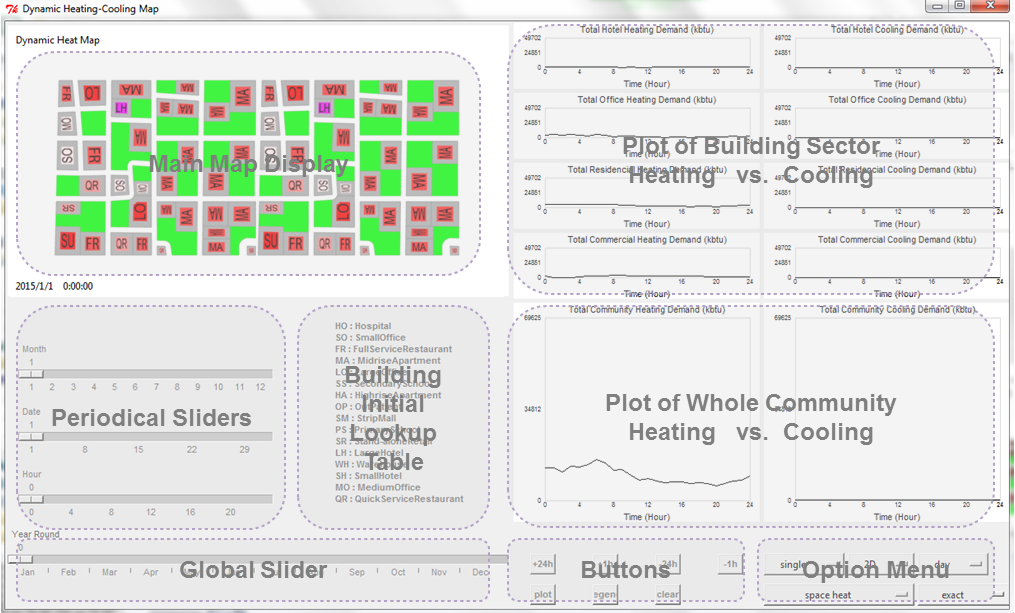
\includegraphics[width=\linewidth]{layout08.png}
  \caption[Dynamic Energy Map Interface Layout]{Dynamic Map Interface Layout}
  \label{fig:layout08}
\end{subfigure}
\caption{Dynamic Map Interface Layout}
\label{fig:interfaceLayout}
\end{figure}

\begin{itemize}
\item A main map display on the upper left that shows the 2D or 3D
  version of the dynamic energy map with energy data encoded as the
  color of buildings. 

\item Four sliders that controls the linear and periodical navigation
  of the map image display and data plot.

\item A ``Building Initial Look-up Table'' in the center bottom that
  defines the two-letter building type initials on the main map
  display window.
\item A series of energy demand plots for four major building sectors
  (top right) and the whole community (lower right).  
\item A series of buttons and option menus on the lower right. 

  The top row of the buttons performs forward (+) or backward (-) time
  navigation with time step of 24h or 1h. The bottom row of the
  buttons contains a ``plot'' button that plots the energy profile
  graphs of the 16 benchmark buildings (if ``single'' is chosen for
  option menu'') or the plot of the aggregated community (if
  ``community'' or ``group'' is chosen), a ``legend'' button that
  shows the current legend, and a ``clear'' button that clears the
  selection in the 2D mode.
\end{itemize}

The following sections will provide more detailed explanation of the
interface.

\subsection {Main Display Window} \label{2d3d} 

As is mentioned in ~\cite{Brownrigg2005}, the choice of 2D
representation vs. 3D representation is one of the debated decisions
in the world of cartographic data
visualization~\cite{Brownrigg2005}. 2D maps are 1) easier to navigate
and 2) the operation of selecting an element or a region is easier to
perform in a 2D map. Another important advantage of 2D map is that it
has better theory support~\cite{Resch2014}: Jacques Bertin defined the
seven visual variables in the graphic sign-system and their
construction rules to effectively convey geographic information
~\cite{Bertin1983}. However the principles and variables of 3D or 4D
maps (space-time map) are not thoroughly
investigated~\cite{Resch2014}. This situation makes the design of 3D
maps more difficult. However 2D maps ``drastically simplify reality
and thus do not give credit to the highly complex capabilities of
human spatial cognition''~\cite{Resch2014}. Regarding this, a 3D map
is rich in geometry representation and can provide realistic
scenes. The realistic scene is important in conveying information to
not only researchers but also the general public. The difference in
surrounding building height and their exterior reflection properties
could influence the exterior shading of a building, so the height and
density distribution of a community could influence its total energy
demand. The correlation of 3D community configurations with difference
in building height, density and exterior surface properties on the
total community level energy performance could also be identified with
a 3D display. The current project does not use the whole-community
energy simulation and this capability of the 3D display is not
demonstrated. Integration with whole-community simulation thus could
be one of the later development of the current project. However, the
3D display can both be an advantage or disadvantage based on the
actual map usage. According to Tufte's data-ink ratio theory, the
extra non-crucial richness of information should be eliminated to make
the most important information stand out~\cite{Tufte83}. For an energy
map, variables such as geothermal energy potential, biomass potential
could be represented as 2D layers while solar energy potential might
be more suitable to be visualized in 3D layers since its performance
is influenced by exterior shading in an urban environment.

For the current dynamic energy map interface, both 2D and 3D
representations are provided for the users to select.  The main map
display window on the top left is used for displaying the 2D / 3D
dynamic map of the conceptual model. The lower left of the main map
display window displays the current time for the image and data
plots. By selecting the 2D / 3D option in the option menu on the lower
right, the user can choose between 2D and 3D display. The 3D display
provides a more realistic view of the community model. The building
geometry is simplified in the current model in order to emphasize the
color changing between frames without introducing distraction from
complicated building geometry. Additional building details or features
could be added to make the display more realistic. In the 2D display,
the user can click on a single building or select a group of buildings
to display their energy profile plots or the aggregated energy profile
plots (\fref{fig:2d3dSelect}).

\begin{figure}[h!]
  \centering
  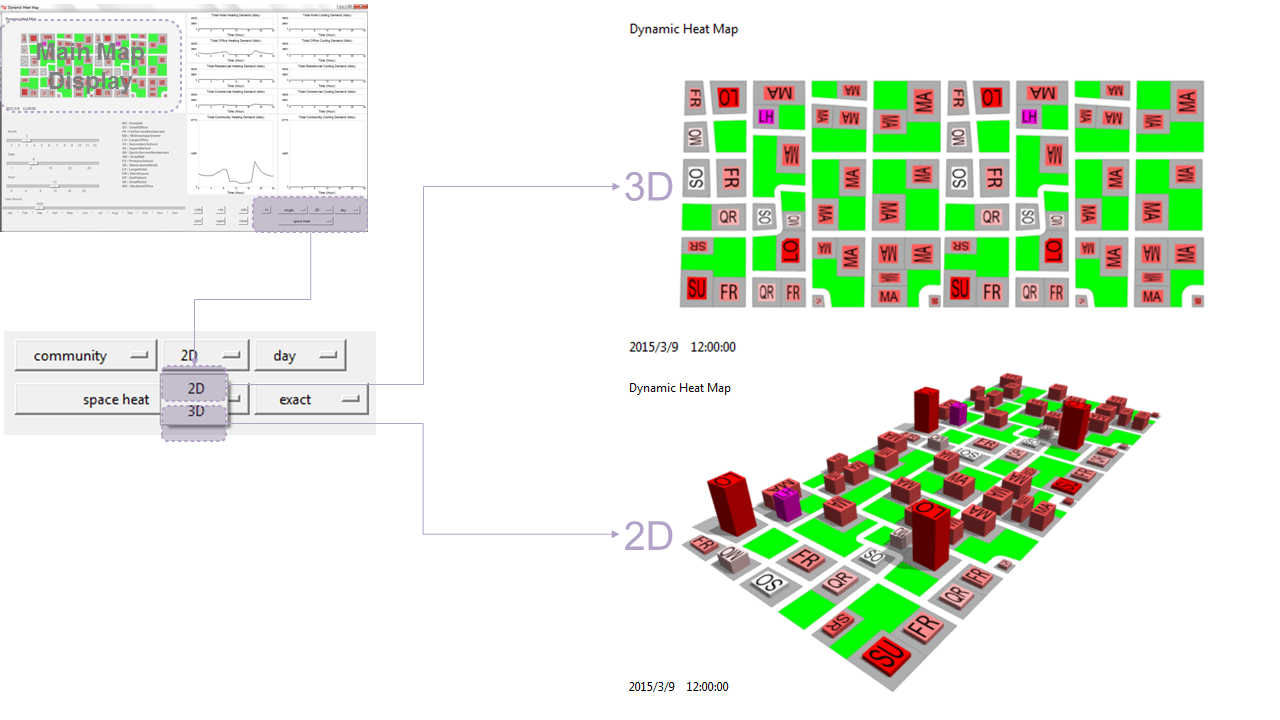
\includegraphics[width=0.7\linewidth]{2d3dSelect.png}
  \caption[Map Display of 2D and 3D]{The current interface provides
    the choices of viewing 2D and 3D map display by toggling the 2D/3D
    option menu}
  \label{fig:2d3dSelect}
\end{figure}

\subsection{Bivariate Map Legend} \label{bivariate}

\subsubsection{Symbol Chosen}
The major reason for choosing the 3D energy dynamic map display is to
use it to provide a more realistic urban environment context.  In the
Dutch Heat map by Dobbelsteen et al.\ , the quantity of energy demand
of each building or region is represented by extruding the building or
region by a corresponding height encoding its energy demand or supply
~\cite{Dobbelsteen2013}. This approach provides an easy way of
aggregating energy demand and supply by adding up geometry height. For
this project this approach was not chosen for the map design because
it creates shape distortion and will impair the goal of providing a
realistic urban environment vision.

In order to represent space heating demand and cooling demand on the
same map, a common map design case is encountered in the current
project: bivariate map design that visualizes the correlation of two
variables on a same map. Elmer points out the challenge of the
bivariate map design as a result of its increased information
density. He presented eight possible types of representation for
bivariate maps (\fref{fig:bivariateExp}): ``shaded cartographer,
rectangle map, bar chart, value by alpha, choropleth with graduated
symbol, bivariate choropleth, spoke glyph and shaded
texture''~\cite{Elmer2012}. In order to incorporate the bivariate map
symbols to the current 3D model without introducing too much shape
distortion, the researcher did not choose the representation with
dimensional changes, i.e. the changing of building height, width,
depth or the size changing of building centroid are not chosen in the
map design of the current project. The choices are the ones that
involves color or texture, i.e. ``bivariate choropleth, value by alpha
and shaded texture'' (\fref{fig:bivariateExp}). Among these three
choices, bivariate choropleth representation has the highest accuracy
rate~\cite{Elmer2012}, hence the researcher chose bivariate choropleth
as the representation of the current map interface design.

\begin{figure}[h!]
  \centering
  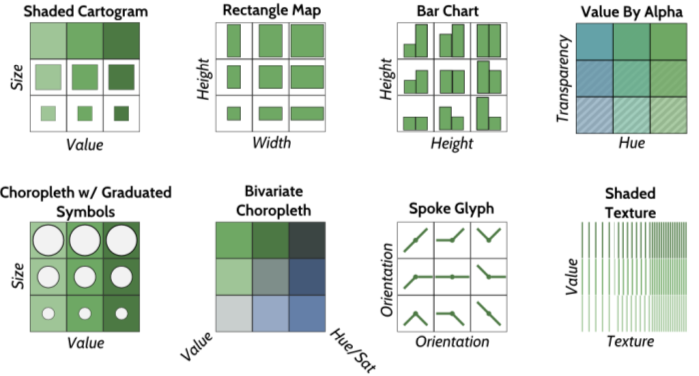
\includegraphics[width=0.7\linewidth]{bivariateExp.png}
  \caption[Bivariate Map Symbol Tested]{The eight bivariate map
    display approaches tested in Elmer's~\cite{Elmer2012} study}
  \label{fig:bivariateExp}
\end{figure}

\begin{figure}[h!]
  \centering
  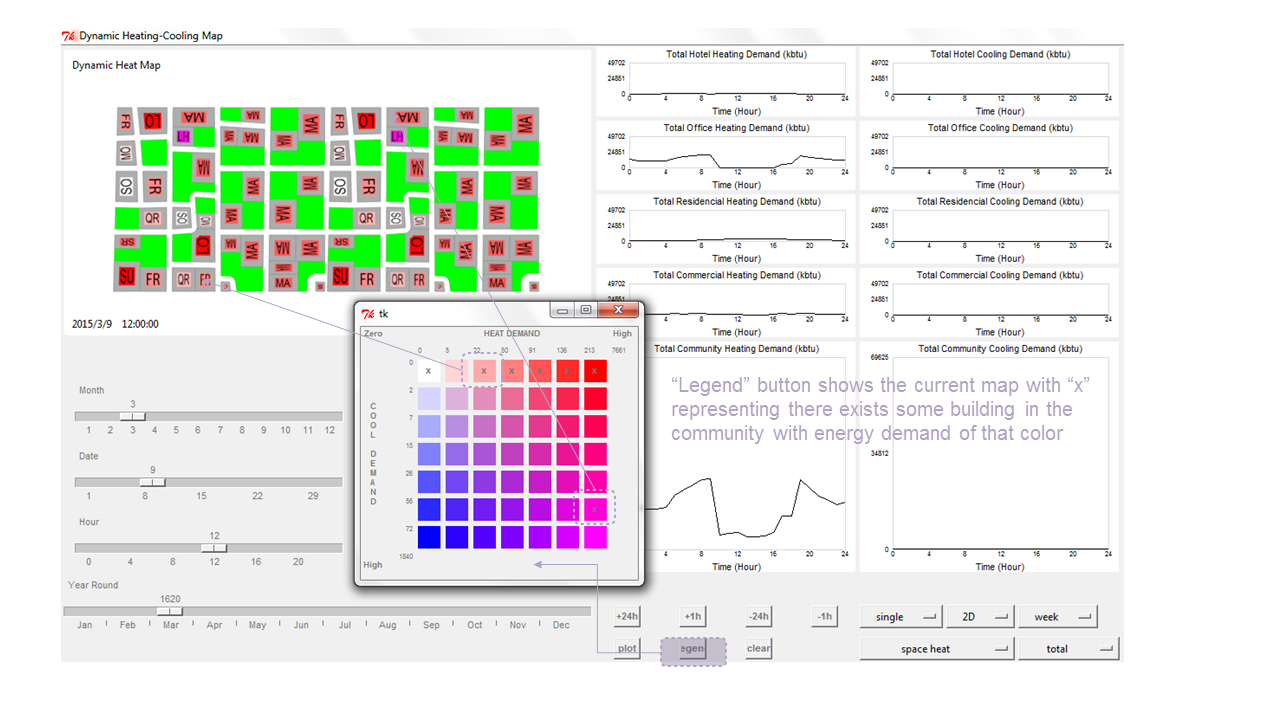
\includegraphics[width=0.7\linewidth]{legend.png}
  \caption[Bivariate Map Legend]{The seven-class-bivariate choropleth
    legend is used in the dynamic energy map interface design with red
    representing high space heating demand, blue representing high
    space cooling demand. ``x'' in the legend corresponds to colors
    appear in the current map display window}
  \label{fig:legend}
\end{figure}

In the current interface design, users can click on the ``Legend''
button and a legend used for encoding the 2D and 3D map will be
displayed. To assist legend reading and color comparison between the
map and the legend, tick marks of ``x'' are added to the legend to
indicate the color appeared in the map \fref{fig:legend}. How to use
the legend to identify the buildings or building groups that have
large energy recovery potential is demonstrated in \sref{useCase1}.

\subsection{Time Sliders and Navigation Buttons}
The lower left section contains a series of sliders for controlling
interactive navigation of the image sequence and the corresponding
data plot.

Harrower and Fabrikant classify time into two types: linear and
cyclic~\cite{Harrower2008}. The former represents the periodical
changes and the latter represents the linear changes of spatial
temporal variables. To address this, the design of the current
interface includes both an overall time navigation utility and time
navigation utilities that facilitate jumps with time steps
corresponding to the natural period of energy data, such as month, day
and hour. This design choice is anticipated to facilitate the
representation of both linear changes and periodical changes of energy
usage in the community.

There are three shorter ``periodical'' sliders on the lower left of
the interface. One unit of position change in the ``month'' slider
results in a forward or backward jump of one month in time. The total
number of positions in the ``month'' slider equals the number of
months in a year (which is the next level of time unit regarding
month).  The jump step for ``date'' slider is one day and the number
of positions in the ``date'' slider is the number of days per
month. Similarly for the ``hour'' slider, the jump step is one hour
and the number of positions in the ``hour'' slider is the number of
hours per day. Suppose the current time in display is 2015/1/1
12:00:00. By moving the month slider, viewers can see the energy
demand in the form of map image and data plot for 2015/2/1 12:00:00,
2015/3/1 12:00:00, $\dots$, 2015/12/1 12:00:00. Similarly, if viewers
pull the ``date'' slider, they can compare the different energy demand
of this hour (12:00:00) throughout the whole month. With the hour
slider, viewers can compare the energy demand between different hours
of a day.

There is a longer ``linear slider'' on the bottom left of the
interface. It has a time step of an hour and a navigation range of a
year (8760 hours). It allows users to globally navigate through all
8760 hours of the year.

There are four buttons (+24h, +1h, -24h, -1h) on the bottom right of
the interface. They provide a micro level adjustment of time.

\subsection{Data Plot}
\subsubsection{Methods to Show Plot}
There are three ways to view energy data plots in the dynamic energy
map interface:
\begin{enumerate}[1)]
\item \textbf{By viewing the right hand side of the interface.}

  The dynamic data plots are directly shown on the right of the
  interface. They depict the energy demand of the four major building
  types (Hotel, Office, Residential and Commercial buildings) and the
  community.

  Space heating and cooling energy demand is displayed in
  \fref{fig:interfaceLayout}. The interface can also display the
  electricity and heating demand for the CHP plant sizing
  application. These plots starts from the current time showing on the
  time sliders with a fixed plotting range of 24h.

\item \textbf{By clicking on the ``plot'' button on the lower right of
    the interface.}

  If the ``single'' option in the option menu is chosen before one
  clicks the ``plot'' button, a data plot will be created for each
  building type (\fref{fig:singlePlot}). If the ``community'' option
  in the option menu is chosen before one clicks the ``plot'', a data
  plot for the community will be created (\fref{fig:communityPlot}).

  \begin{figure}[h!]
    \centering
    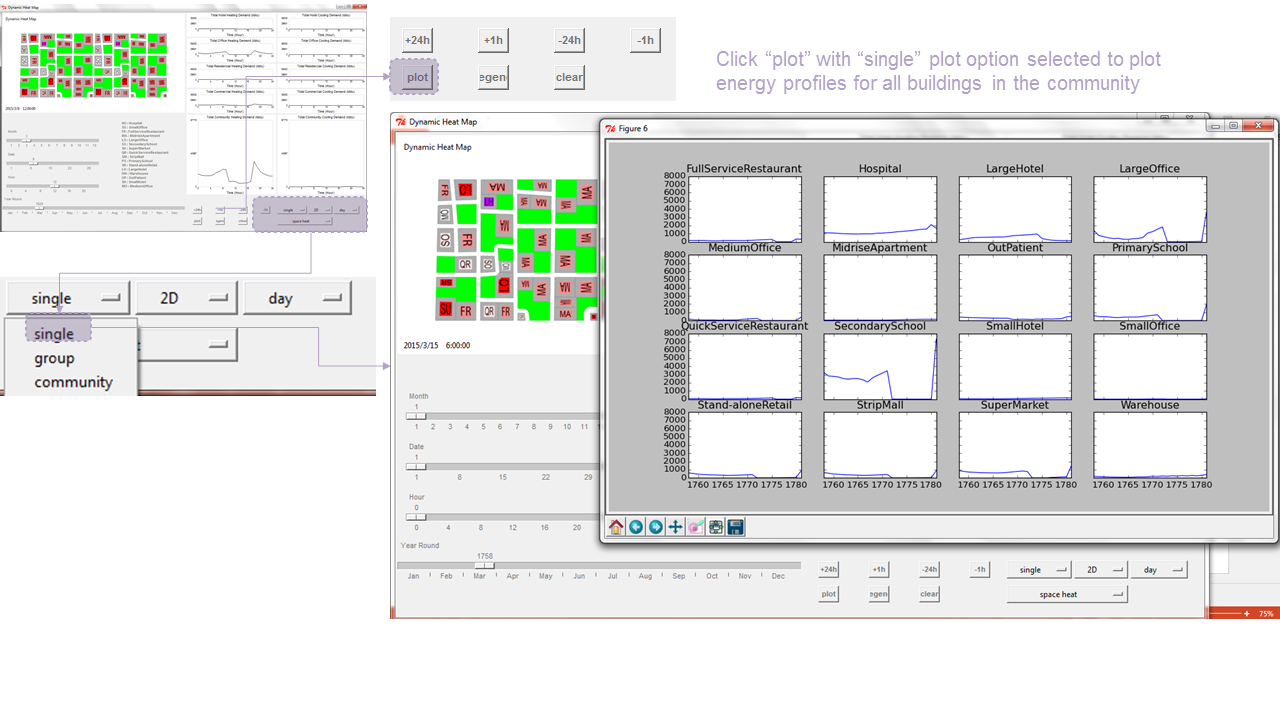
\includegraphics[width=0.9\linewidth]{singlePlot.png}
    \caption[Single Plots of 16 Building Types]{The plot shows the
      space heating energy demand plot of each of the 16 benchmark
      buildings}
    \label{fig:singlePlot}
  \end{figure}

  \begin{figure}[h!]
    \centering
    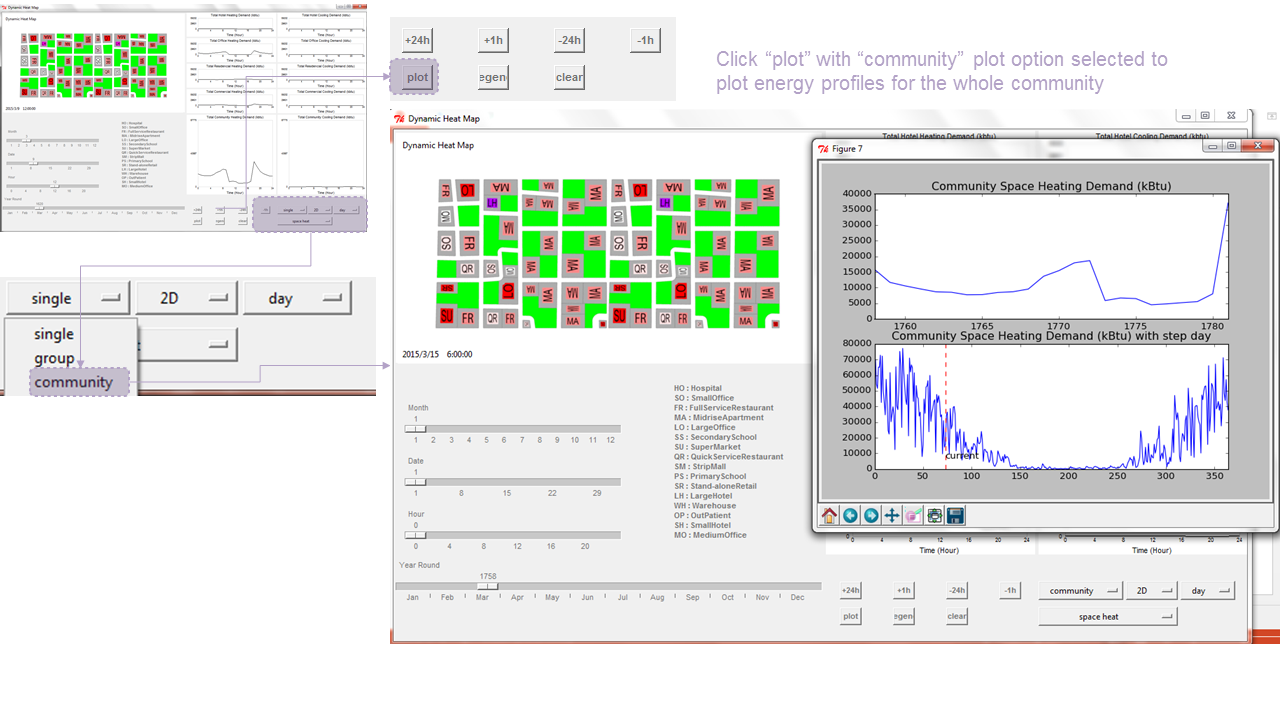
\includegraphics[width=0.9\linewidth]{communityPlot.png}
    \caption[Community Plot]{The plot shows the aggregated space
      heating energy demand for the whole community}
    \label{fig:communityPlot}
  \end{figure}

\item \textbf{By clicking on the building footprint in the 2D map
    display.}

  A building is ``selected'' if the user clicks on its foot
  print. Each new click of a building footprint will add a new copy of
  that building to the selection set. The selection set can be cleared
  by pressing the ``clear'' button. If ``single'' option is chosen in
  the option menu before clicking on a building's footprint, a data
  plot will be created for the building the viewer just clicked on
  (\fref{fig:clickSingle}). If ``group'' is chosen in the option menu,
  each click of a building's footprint will create a data plot for the
  current selection set (\fref{fig:clickGroup}). This function is
  important in assessing the building group level energy recovery
  potential. Users can assess the energy recovery potential of the
  building or building group that rejects heat. They can also assess
  the space heating demand of the group of surrounding buildings of
  the reject heat producers. By comparing these two graphs the users
  can assess the effectiveness of energy recovery strategy in reducing
  the space heating demand of the group of buildings. A demonstration
  of presented in \sref{useCase1}
  
  \begin{figure}[h!]
    \centering
    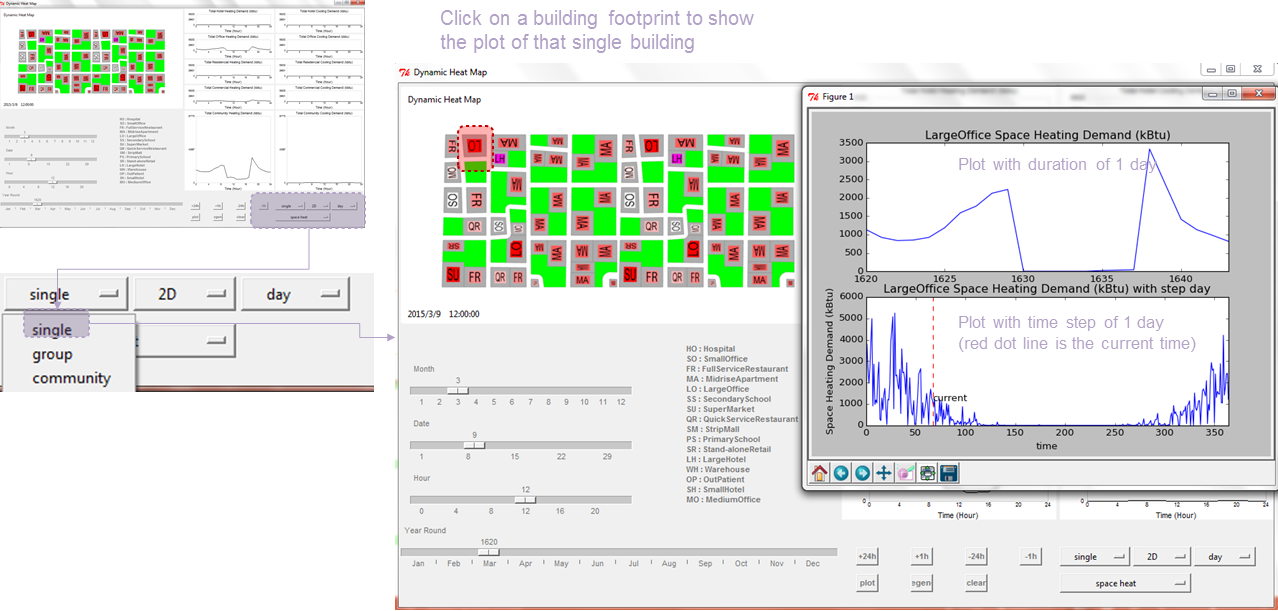
\includegraphics[width=0.9\linewidth]{clickSingle.png}
    \caption[Show Plot for One Building]{Click on a building foot
      print shows the energy plot of this building}
    \label{fig:clickSingle}
  \end{figure}

  \begin{figure}[h!]
    \centering
    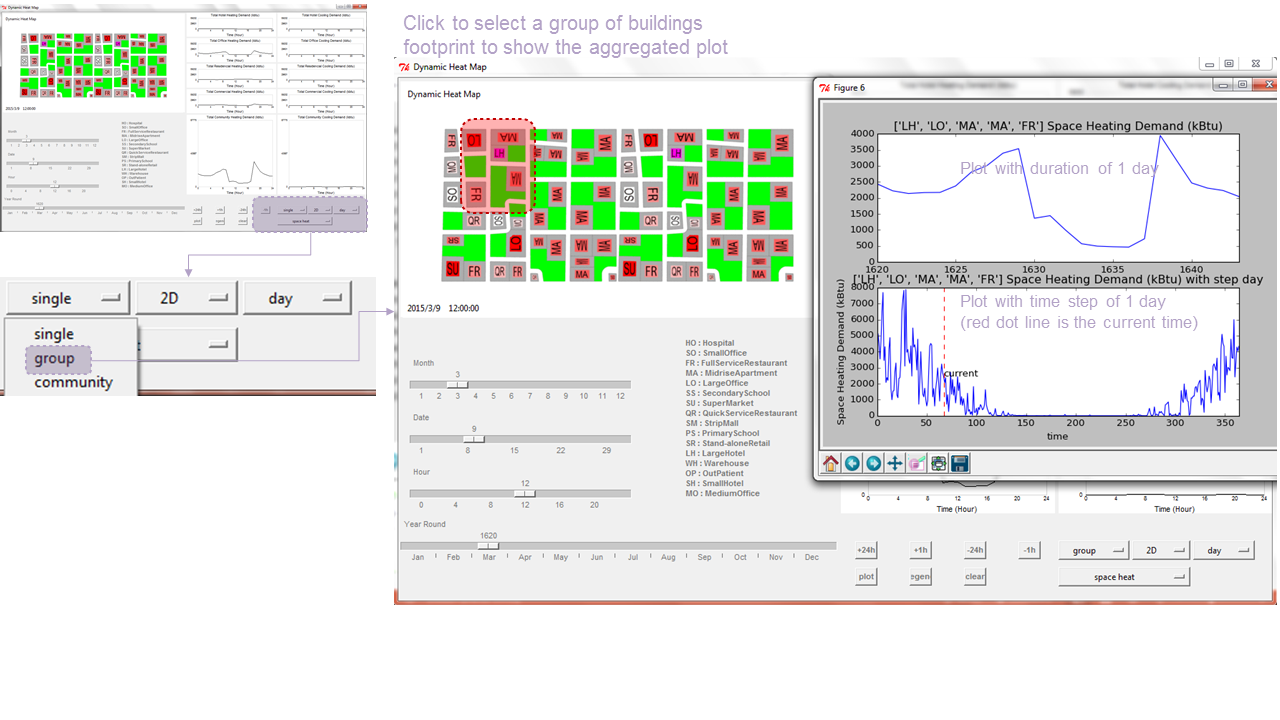
\includegraphics[width=0.9\linewidth]{clickGroup.png}
    \caption[Show Plot for a Group of Buildings]{Click on a building
      footprint shows the energy plot for the selected building group}
    \label{fig:clickGroup}
  \end{figure}

\end{enumerate}

\subsubsection{Providing Temporal Context in Data Plot}

Brownrigg suggested that it is necessary to provide a temporal context
in a space-time map: ``To comprehend how drastically or subtly
something is changing, how fast or slow, in what direction, in
relative to its environment, etc., demands some knowledge of the
history of the change, an awareness of the objects' properties before
and after the change.''~\cite{Brownrigg2005}.

In the current map image display, the temporal context is created by
providing three ``periodical'' slider bars that allows the user to
jump with time steps of month, day and hour. 

In data plots, the temporal context is created by providing a
``longitude'' and ``latitude'' comparison of energy demand.
``Longitude'' here refers to the comparison of adjacent time spots. It
shows what the states of the direct future or past comparing to the
state of the current time. ``Latitude'' here refers to the comparison
of the current time spot with all similar time instances, for example,
all 12:00:00 energy demand of the year. It shows how the current
instance differ from similar instances.

For the current interface design, the top plot presents a longitude
temporal context of the energy demand of the incoming 24h, week or
month. Corresponding to the duration of time of the top plot (24h or
one week or one month), the bottom plot presents the latitude demand
context of the same hour with a step of one day, one week or one
month. For example, in \fref{fig:dayContext}, the top plot shows the
Space Heating Demand for Large Office from 2015/3/9 12:00:00 to
2015/3/10 11:00:00, with a duration of 24h. The bottom plot shows the
energy demand of the Large Office for all 12:00:00 of the 365 days of
the year (the red dot line indicates the 12:00:00 of around the 70th
day of the year, which is the date of Mar. 9th).

\begin{figure}[h!]
  \centering
  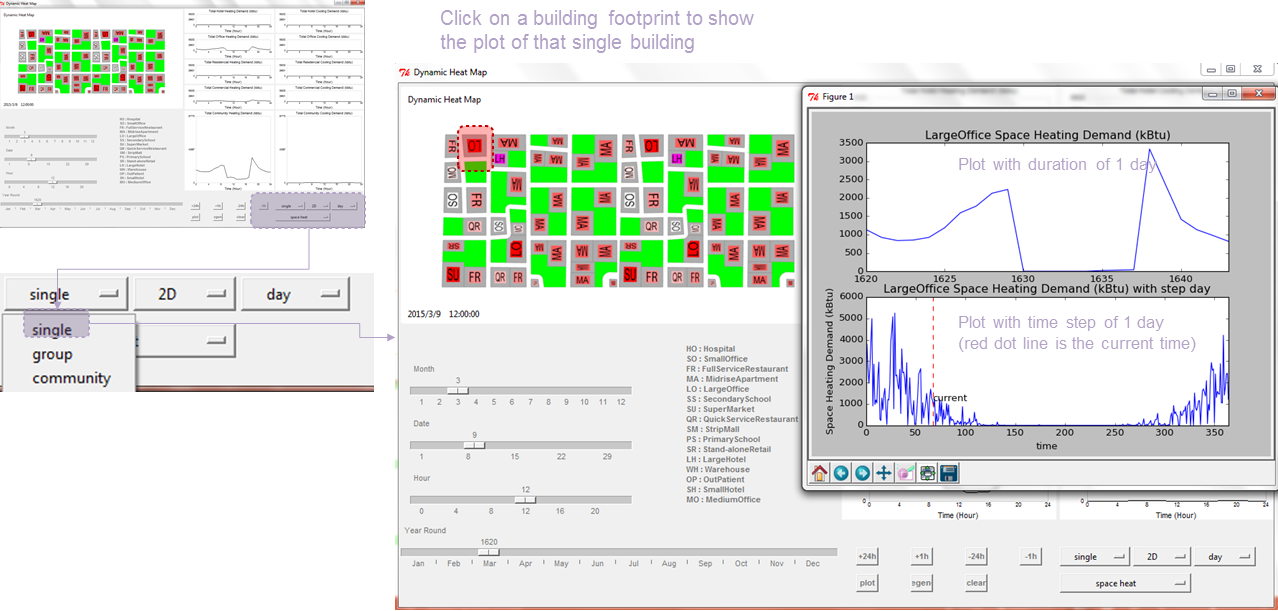
\includegraphics[width=0.9\linewidth]{dayContext.png}
  \caption[Data Plot with Duration / Step of One Day]{The data plot
    presents the longitude and latitude comparison of energy demand,
    the top plot presents a temporal context of the energy demand of
    the next 24h, the bottom plot presents the time context of the
    demand of the same hour throughout the 365 days of the year}
  \label{fig:dayContext}
\end{figure}

\begin{figure}[h!]
  \centering
  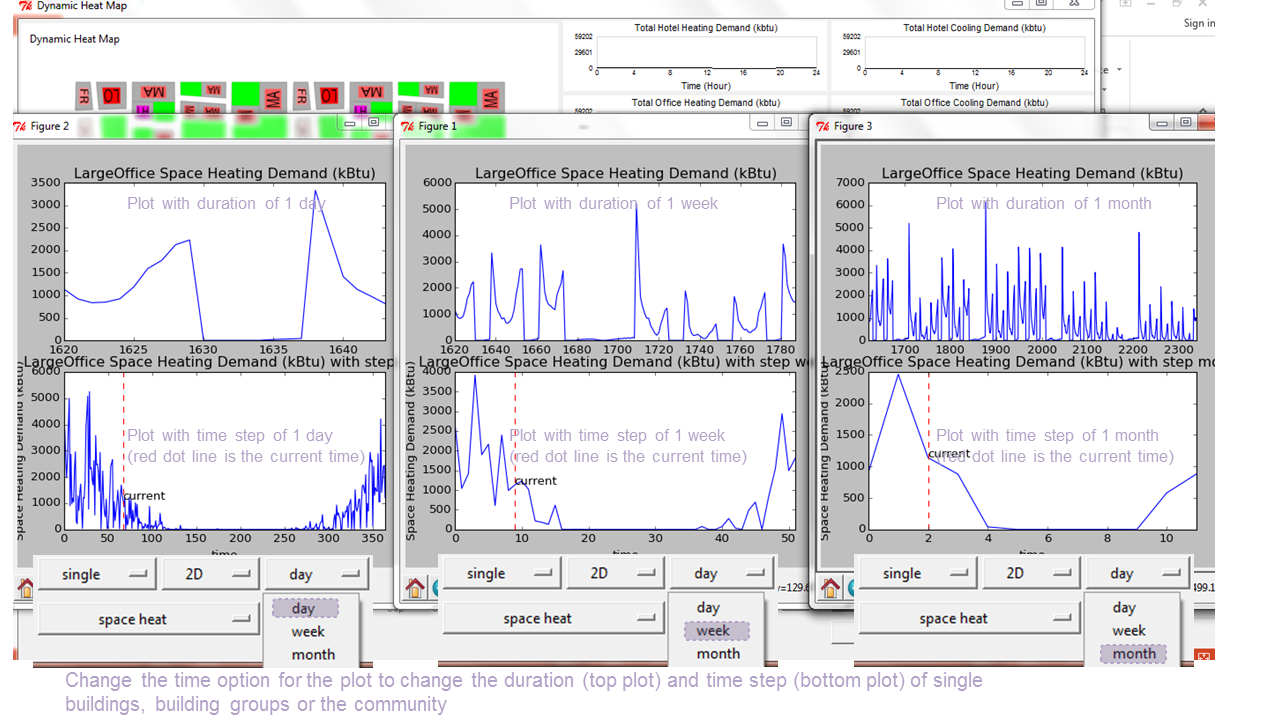
\includegraphics[width=0.9\linewidth]{changeT.png}
  \caption[Data Plot with Different Duration / Step]{By changing
    option in the option menu. User can choose to display a longitude
    latitude comparison with the time unit of day, week or month. The
    top plot shows the energy demand for the next day, week and month
    from left to right; the bottom plot shows the energy demand of
    this hour in the 365 days of year, 52 weeks of a year or the 12
    months of a year from left to right}
  \label{fig:dayContext}
\end{figure}

By providing the temporal context, the viewers are provided with a
general understanding of whether the changing of energy demand
behavior is drastic or subtle and whether a drastic change is coming
and whether the current demand is high, low or moderate comparing to
the overall distribution over time and space.

\pagebreak
\section{Use Case Demonstrations}
\subsection{Use Case I: Identification of Energy Recovery Opportunity}\label{useCase1}
In this section, the researcher present a general approach on how to
use the dynamic energy map interface to identify the energy recovery
opportunities. The process of space cooling will produce reject
heat. As is explained in \sref{sec:inputRecover}, the ammount of
cooling-induced reject heat is positively corelated to the cooling
demand. Thus a building with high cooling demand will also have a
large amount of reject heat. The reject heat from this building or
group of buildings could possibly be recovered for use within the
building such as pre-heating water or outside air or be transmitted to
other buildings that have space heating demand so that the total space
heating demand of the group of buildings could be reduced.

For the interface design in the current study, the researcher used a
bivariate color ramp in space heating and cooling energy demand data
representation that depicts the hourly space heating and space cooling
demand on the same map (\fref{fig:legend2d}) . Red represents high
heating demand and blue represents high cooling demand. The closer the
color cell is to the top, the lower cooling demand. The closer the
color cell is to the left, the lower heating demand. The cells on the
diagonal line (purple colored cells) represent buildings that have
relatively similar heating and cooling demand. The cells to the upper
right of the diagonal represents buildings that are heating dominated
and the cells to the lower left of the diagonal represent buildings
that are cooling dominated. The current breakpoints are decided
through the ``Quantile method'' ~\cite{GIS_Jenks2014} for
demonstration.

\begin{figure}[h!]
  \centering
  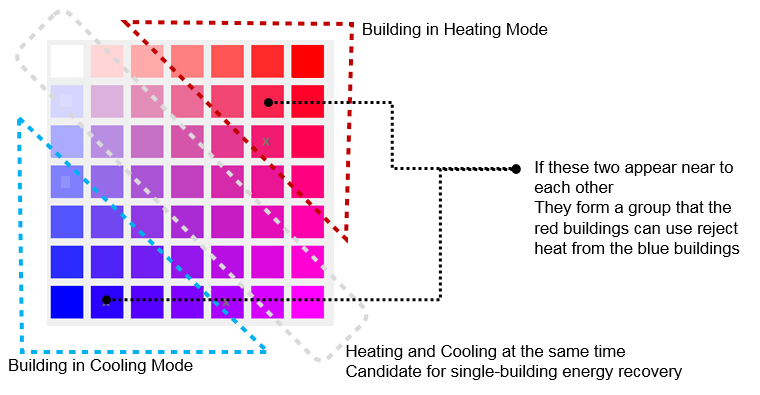
\includegraphics[width=0.7\linewidth]{legend2d.png}
  \caption[Heating-Cooling Map Legend Illustration]{The bivariate
    color ramp displays two variables at the same time: space heating
    and space cooling. It better displays the co-relation between
    these two variables and thus helps users to identify energy
    recovery opportunities}
  \label{fig:legend2d}
\end{figure}

With the dynamic energy map, the buildings colored in one of the
colors in the bottom rows of the legend are buildings with high
cooling demand. With the dynamic energy map, users can identify the
potential reject heat suppliers and consumers over time
(\fref{fig:highCooling}).

\begin{figure}[h!]
  \centering
  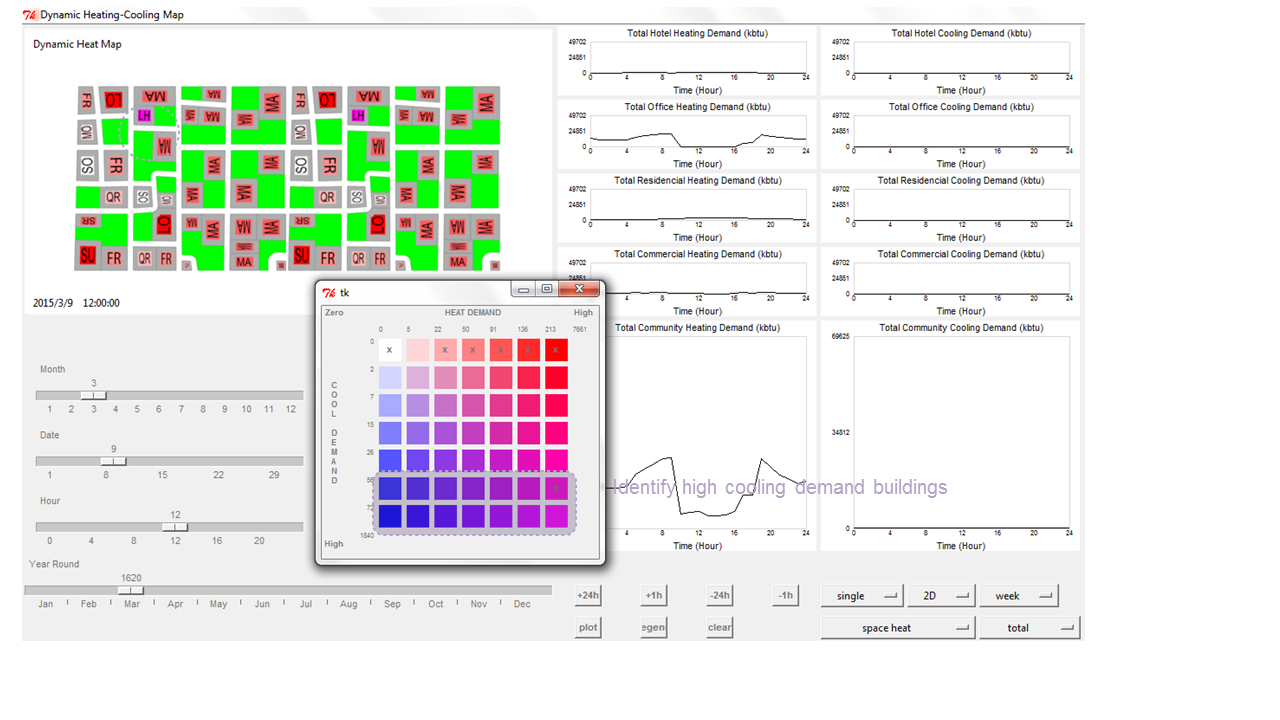
\includegraphics[width=0.7\linewidth]{highCooling.png}
  \caption[Identify Buildings with High Cooling Demand]{In the
    demonstration, buildings with a high cooling demand have colors on
    the bottom rows of the legend, thus Large Hotel and Large Office
    are identified as potential reject heat energy suppliers}
  \label{fig:highCooling}
\end{figure}

Users can then calculate the ``energy recovery potential'' in the
dynamic energy map with a specified time duration and step.  In the
example of \fref{fig:ERP}, users identify the Large Office and the
Large Hotel as reject heat suppliers and calculated their aggregated
energy recovery potential for the 16th week of the year in the graph
on the left. Then they calculated the space heating energy demand of
the group of surrounding buildings of reject heat suppliers: two First
Service Restaurants, two Midrise Apartment and one Small Hotel. 

By comparing the two graphs, users can see that the peak of the energy
recovery potential is about four times of the peak of the space
heating demand of the group of surrounding buildings. They can also
observe that there are two peaks for space heating demand of the
surrounding building group but only one peak for the energy recovery
potential. There are some difference in the weekly pattern of the
reject heat supply and the space heating demand: the last two days of
the week has very little reject heat but the space heating demand is
relatively high. We can also see that the peak of reject heat does not
occur at the same time with the space heating demand peak: in the
2800th hour, reject heat (in the graph on the left) reaches its peak
while space heating demand on the right is zero. With the dynamic
energy map, users can identify complicated non-coincidence in the
supply and demand of reject heat. This information could help users
conduct more detailed heat recovery strategies and assess the thermal
energy storage devices.

\begin{figure}[h!]
  \centering
  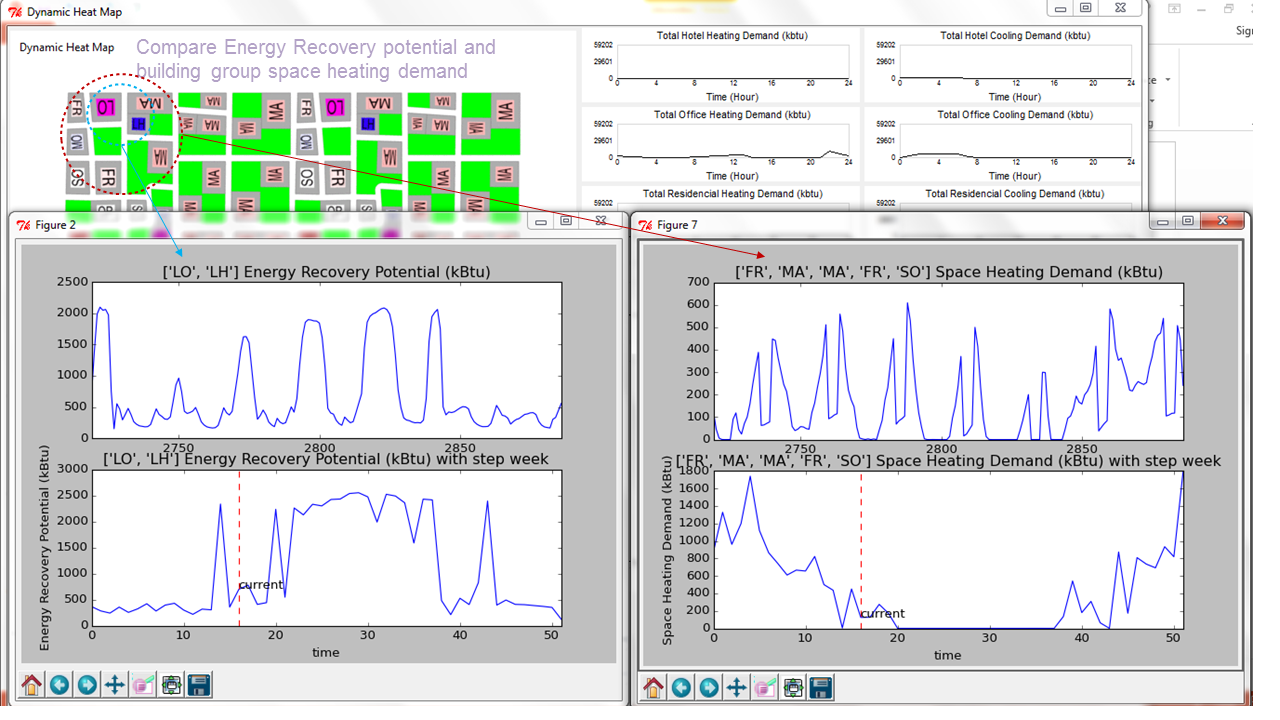
\includegraphics[width=0.7\linewidth]{ERP.png}
  \caption[Calculate Energy Recovery Potential]{The users can
    calculate the energy recovery potential of the group of reject
    heat suppliers (Large Office and Large Hotel). They can also
    calculate the total heat demand of the surrounding buildings with
    space heating demand (two FirstService Resturant, two Midrise
    Apartment and one Small Office).}
  \label{fig:ERP}
\end{figure}

\subsection{Use Case II: Sizing CHP Plant}
With the Dynamic Energy Map that depict the spatial temporal load
variation, one will idealy be able to 1) idendify anchor load
buildings, 2) conduct better design of local load balancing, 3) size
the co-generation CHP plant

\begin{itemize}
\item Identify anchor load buildings
  
  To achieve this function, the map should be able to make the
  building with persistant high heating or cooling demand stand
  out. Thus the color scheme assigns vibrant colors to high demand and
  white to low demand. The break points of ``high'' demand remains to
  be decided in further project development. For the current
  implementation, the break point is acquired with the quantile
  classification method.

  Although with the box plot of heating demand (\fref{fig:SH}), the
  buildings with high consistently high heating demand through its
  high median and 25 percentile, a more intuitive interpretation is
  still needed to convey information to people with less statistical
  background. From the animated version of the dynamic energy map
  (link to 2d map, link to 3d map) the Large Office, the Large Hotel
  and the Midrise Apartment forms a high heat demand region, these
  could be potential locations for making a connection to a district
  system.

  \begin{figure}[h!]
    \centering
    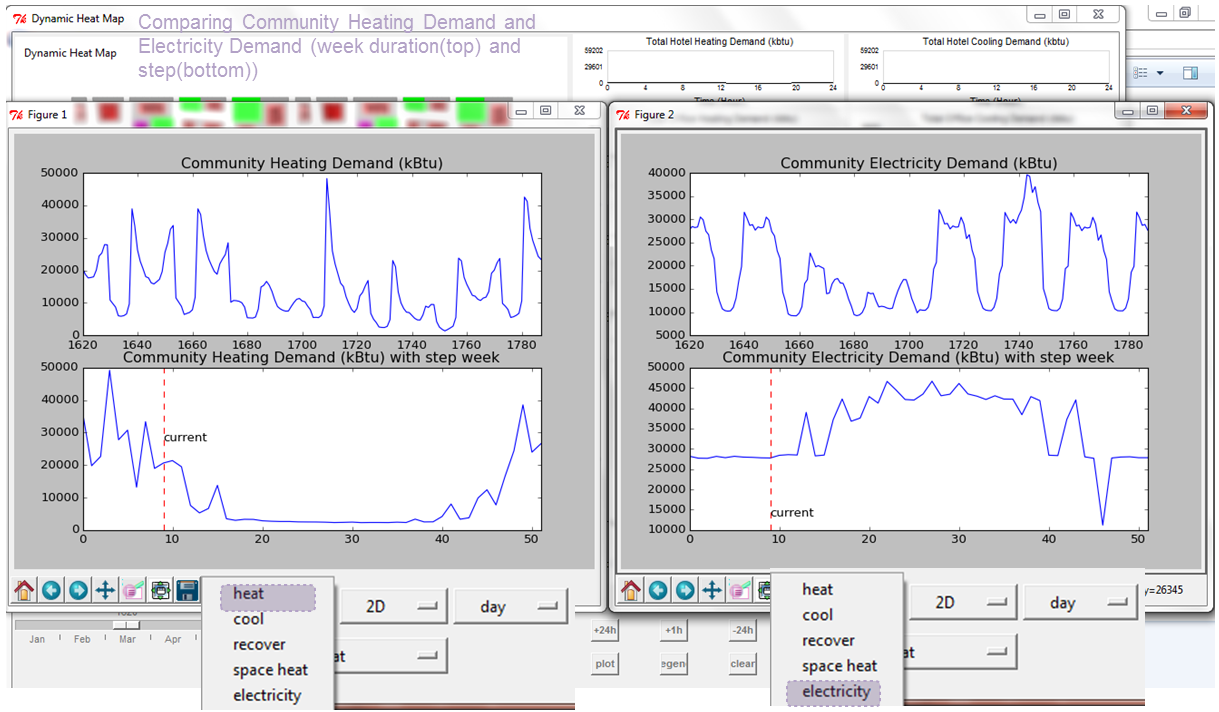
\includegraphics[width=0.7\linewidth]{heatPowerDemand.png}
    \caption[Comparing Community Heating and Electricity Demand]{In
      this example, the users compare the week-wise heating and
      electricity demand}
    \label{fig:heatPowerDemand}
  \end{figure}
\item Size a CHP plant 

  Two variables are crucial in sizing a CHP plant: 1) the heating
  demand including space heating and service hot water 2) electricity
  demand. For the current dynamic energy map interface, a 2D/3D
  choropleth map are presented in the main map display window with the
  heating demand and electricity demand encoded with a seven-class
  bivariate choropleth legend as in \fref{fig:CHPHeating}. The dynamic
  plot on the right of the interface depicts the heating and
  electricity demand of the four building sectors and the community .

  The user can also inspect heating energy and power demand of he
  community with different time span and different aggregation
  method. For example, they can compare the heating and power demand
  for a week and see if the demand align. In \fref{fig:CHPHeating},
  users can see the peak heating demand for the ninth week is about
  the same level as the peak demand for the electricity. However,
  their weekly behavior is different: the heating demand for the
  second half of the week are relatively low but the electricity
  demand is relatively high. The lower graph also shows that the
  annual peak demand of electricity occurs during the time when the
  community has the lowest heating demand. This poses the challenge
  for the district energy system with Co-generation local plant and
  the necessity for thermal energy storage devices in a district
  energy system.

  \begin{figure}[h!]
    \centering
    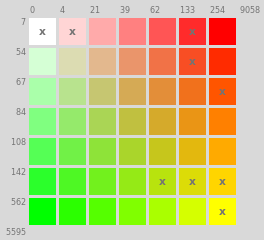
\includegraphics[width=0.3\linewidth]{legendCHP.png}
    \caption[Legend for Heat and Power Map]{Legend for Heat and Power
      Map}
    \label{fig:legendCHP}
  \end{figure}

  \begin{figure}[h!]
    \centering
    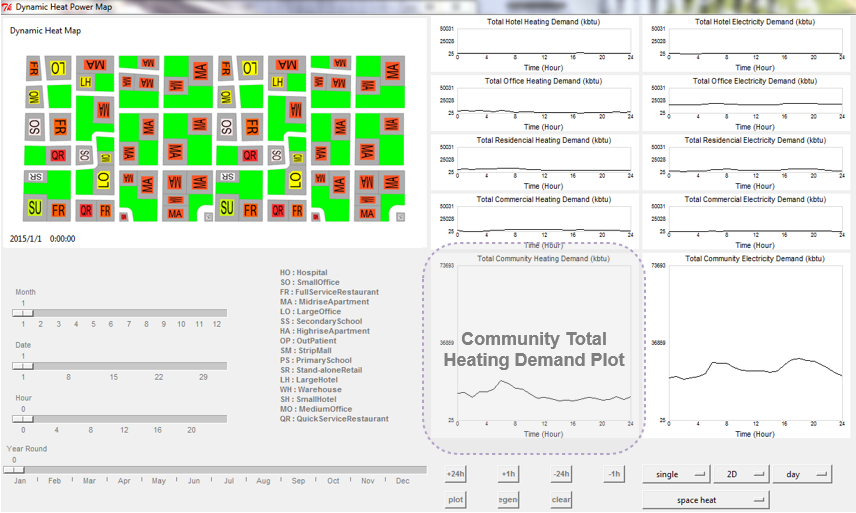
\includegraphics[width=0.7\linewidth]{CHPHeating.png}
    \caption[Interface for CHP Sizing]{In this example, the users
      compare the week-wise heating and electricity demand}
    \label{fig:CHPHeating}
  \end{figure}

\item Local load balancing

  Apart from the information for the minimum and maximum value of the
  heating and electricity demand of the community, more specific
  heating and electricity demand of single buildings and building
  groups are also available. This could be used to design micro-scale
  CHP equipment or to locate thermal energy storage devices and to
  size their storage capacity.  For the micro-scale CHP equipment
  design, a load balancing in the level of a building group could make
  the micro-scale CHP equipment operate in its high efficiency output
  for a longer period.
  
  To achieve this, the program enable users to select a subset of the
  existing buildings and creates the aggregated heating load plot for
  the selected building group (within the specified time period). 

  The user will first identify some cluster of buildings, in which
  there is a pattern of building that turn red sequentially but not
  simultaneously. Then they can check the building demand profile by
  clicking on the building footprint in the 2D map
  (\fref{fig:seeLoad}).

  \begin{figure}[h!]
    \centering
    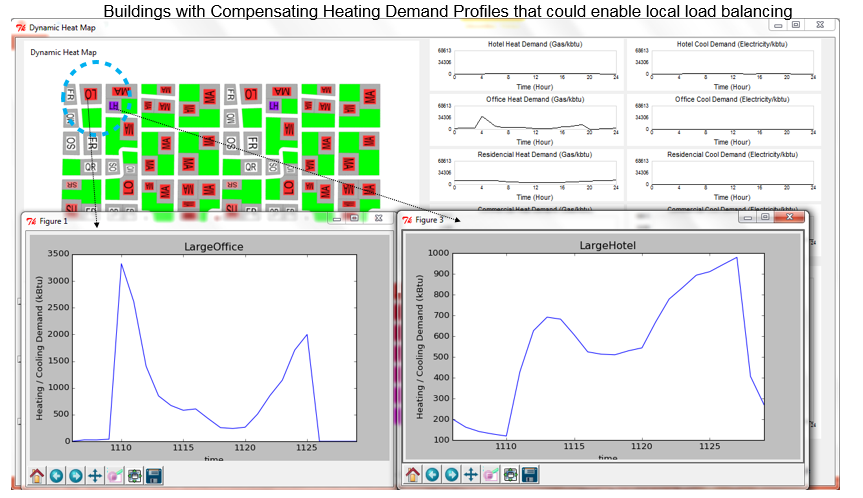
\includegraphics[width=0.7\linewidth]{seeLoad.png}
    \caption[Check Heating Load]{Users can check the building energy
      demand (thermal or electricity) by clicking on the building foot
      print in the 2D map and the interface will show the plot of the
      energy demand profile within a period (the example is showing
      the demand for a 24h hour period)}
    \label{fig:seeLoad}
  \end{figure}

  Alternatively, they can first open the window that displays the 24h
  period energy demand graph (hourly gas heating energy in the
  following example) for all of the 16 prototype buildings and see if
  there are some building types that have demand complimentary (so
  they have a rough idea of what is a ``good building combination''
  (\fref{fig:plotAll}) at this time that could be a candidate for load
  balancing) and they will look at the map and search for this ``good
  combination''.

  \begin{figure}[h!]
    \centering
    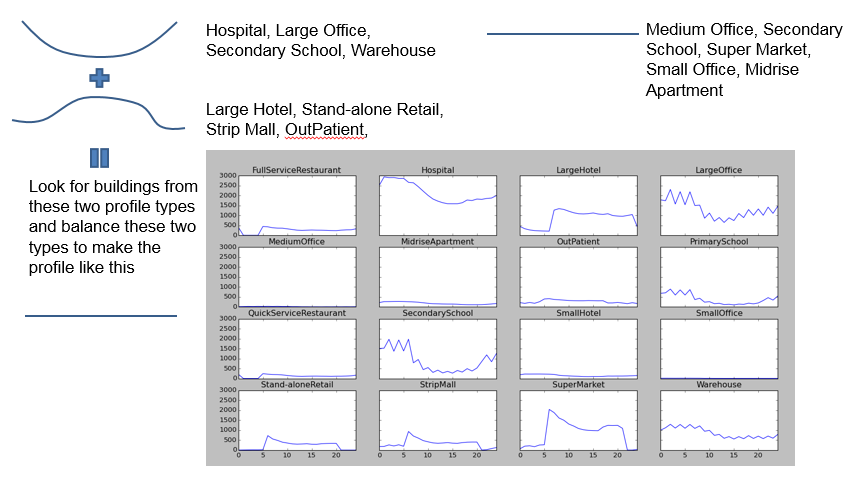
\includegraphics[width=0.7\linewidth]{plotAll.png}
    \caption[Check All Heating Load Plot]{Users can plot all building
      energy demand profile (heating gas demand for the example) and
      search for ``good cobimations'' that have compensate load
      profile}
    \label{fig:plotAll}
  \end{figure}

  After the qualitative experimentation, users can select a group of
  building by clicking on the building footprint and the program will
  output a graph of aggregated load

  \begin{figure}[h!]
    \centering
    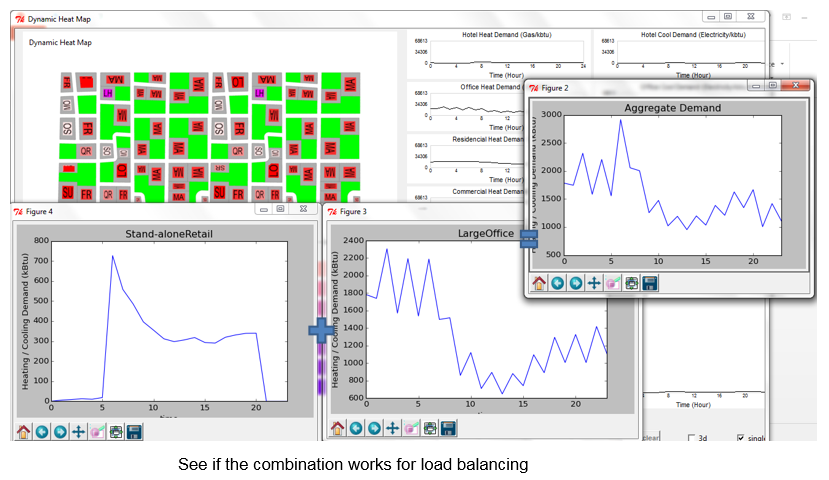
\includegraphics[width=0.7\linewidth]{seeAggDemand.png}
    \caption[Plot Aggregated Demand]{In this example, users selected
      the Stand-alone Retail and the Large Office and plots of each
      single building and the aggregated demand of the two buildings
      are displayed}
    \label{fig:plotAll}
  \end{figure}

\end{itemize}

\begin{comment}
\section{Future Trends}
Harrower and Fabrikant mentioned that the chanllenge of using animated
maps is the overflow of information and the vulnerability to
distraction~\cite{Harrower2008}. One example mentioned by Harrower and
Fabrikant is the comparison of color on the map and that on the legend
becomes difficult for animated maps as a result of the changing of
images. They proposed the audio legend approach of strengthening
information convey with minimized
distraction~\cite{Harrower2008}. This might become one of the next
extensions of the current Dynamic Energy Map interface design.

They also suggested that the difference in time should have different
visual representations in data display~\cite{Harrower2008}. Peuquet
claimed that ``The development of temporal analytical capabilities in
GIS such as temporal queries requires basic topological structures in
both time and space''~\cite{Peuquet1994}. Thus the different spatial
representation seems to be a natural choice for adapting to different
temporal resolution and scale.



The non-interactive animation could be found
\href{http://www.armechxyj.com/energy-mapping.html#redblueAnime3d}{through
  this link}.
\end{comment}